%----------------------------------------------------------------------------------------
%	PROBLEM 1
%----------------------------------------------------------------------------------------

% To have just one problem per page, simply put a \clearpage after each problem
\newpage
\begin{homeworkProblem}
\section{Variable neighborhood descent algorithms}
\subsection{Problem statement}
Implement both a standard and piped variable neighborhood descent (VND) algorithm (concatenation of the underlying iterative improvement algorithms; see lecture slides). Consider the two possible (reasonable) orderings of
the iterative improvement algorithms (indicated by the neighborhood relation they use):
\begin{itemize}
  \item transpose, exchange, insert
  \item transpose, insert, exchange 
\end{itemize}
Implement the 4 VND algorithms (all combinations of standard and piped and the two neighborhood orders) using first-improvement and random initialization.

\subsection{Introduction}
An Iterative Improvement algorithm generally starts from a candidate solution, which can be either generated randomly or using an heuristic, and improves the evaluation of the solution at each step by modifying the solution structure , until a local optimum is reached.

In the previous problem, I considered different kinds of 2-opt neighborhood, and different pivoting rules.

This means that, at each step, a new solution is constructed from the current best by modifying only two solution components (with Transpose,Exchange or Insert operations) and only the first/best improving solution will become the new best soluion.

The main limitation of such kind of algorithms is that they tend to get stuck in solutions that are locally optimum but not globally.

Provided that:
\begin{itemize}
\item A global optimum is optimal with respect to any kind of neighborhood. 
\item A solution that is locally optimal with respect to a neighborhood may not be optimal with respect to other kinds of neighborhood
\end{itemize}
by dynamically changing the neighborhood type an algorithm is able to escape local optima.

This section will analyse the results of the execution of two variable neighborhood descent algorithm, based on the previously analyzed iterative improvement algorithms :
\begin{itemize}
\item \textbf{Standard Variable Neighborhood Descent} (i.e. Changing neighborhood when a local optimum is encoutered, until the neighborhood chain is terminated and going back to the smallest neighborhood every time the local optimum is escaped.)
\item \textbf{Piped Variable Neighborhood Descent} (i.e. Using the locally optimum solution found using one neighborhood type in the chain as the initial solution for the following type.)
\end{itemize}
The same metrics as in \ref{subsec:metric} will be used to evaluate the algorithms.

\subsection{Experiment results}
\subsubsection{n80w20.001}
\begin{center}
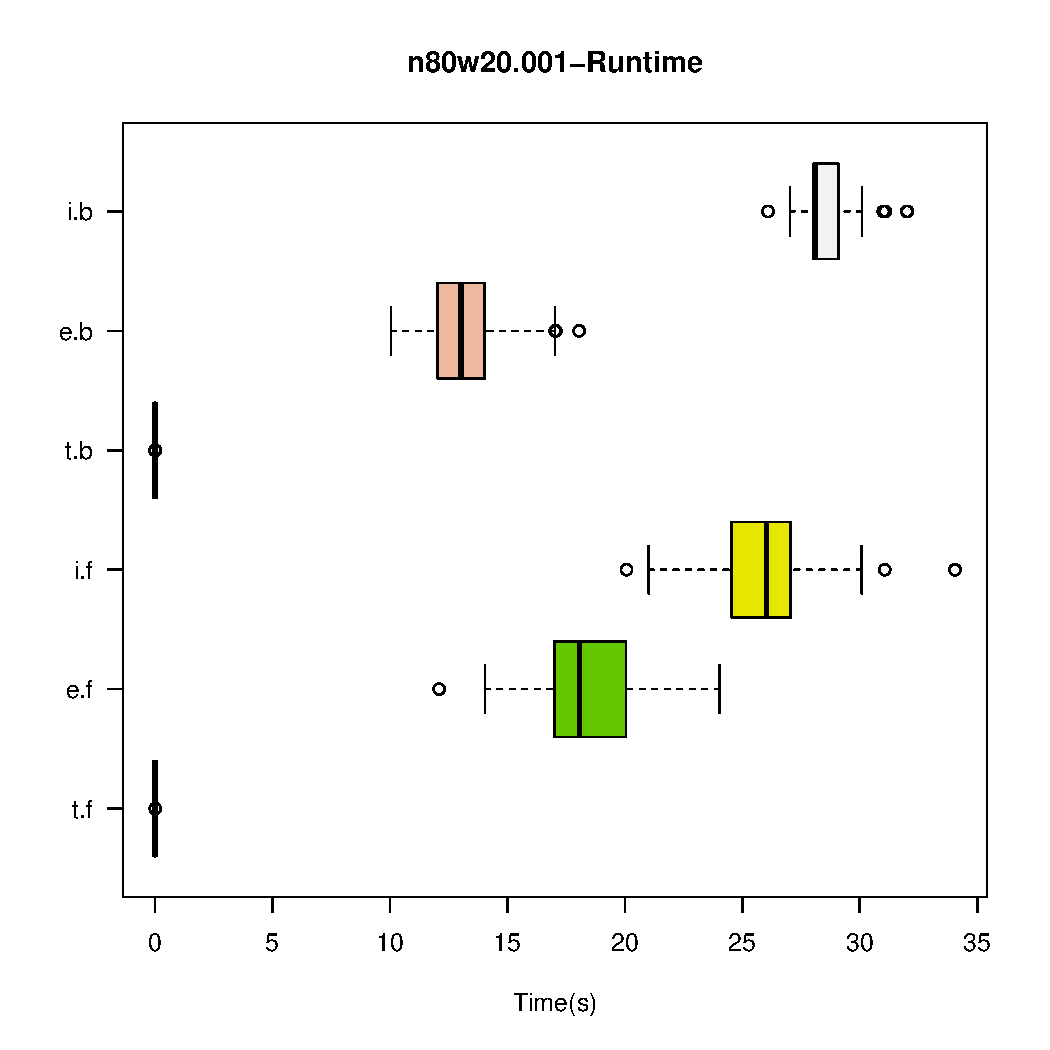
\includegraphics[width=0.6\textwidth,keepaspectratio]{{VND/n80w20.001/n80w20.001-CpuTime}.pdf}
\captionof{figure}{n80w20.001 - Runtime boxplots for the different variable neighborhood descent algorithms}
\end{center}

\begin{center}
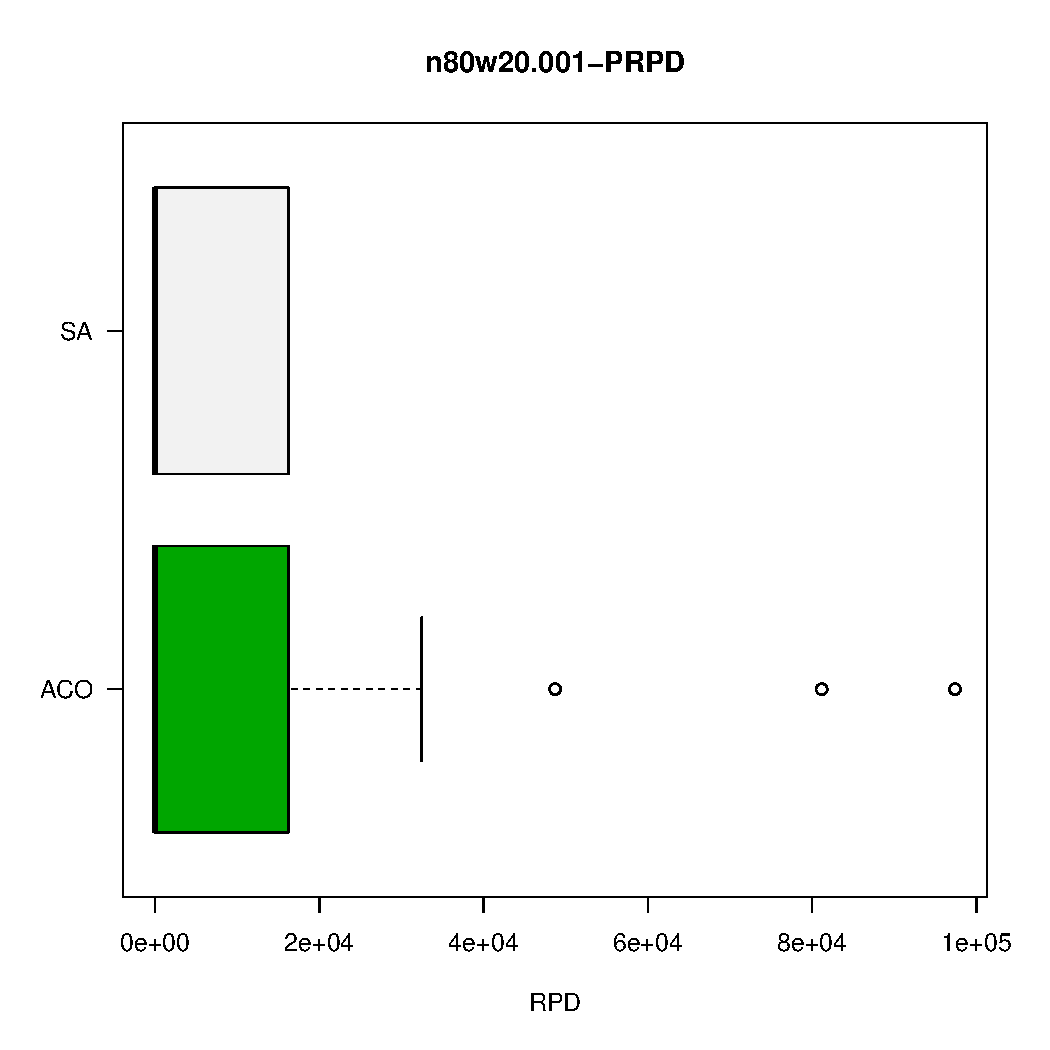
\includegraphics[width=0.6\textwidth,keepaspectratio]{{VND/n80w20.001/n80w20.001-PRPD}.pdf}
\captionof{figure}{n80w20.001 - PRPD boxplots for the different variable neighborhood descent algorithms}
\end{center}

\begin{center}
\begin{tabular}{|l|l|}
\hline
\textbf{Test} & \textbf{P-Value} \\
\hline
Tei vs Tie - Standard&3.95591160889952e-18\\
\hline
Tei vs Tie - Piped&3.9556885406462e-18\\
\hline
Standard vs Piped - Tei&3.95591160889952e-18\\
\hline
Standard vs Piped - Tie&3.95591160889952e-18\\
\hline
\end{tabular}
\captionof{table}{n80w20.001 - Results of Wilcoxon paired signed rank test}
\label{tab:w.11}
\end{center}

\subsubsection{n80w20.002}
\begin{center}
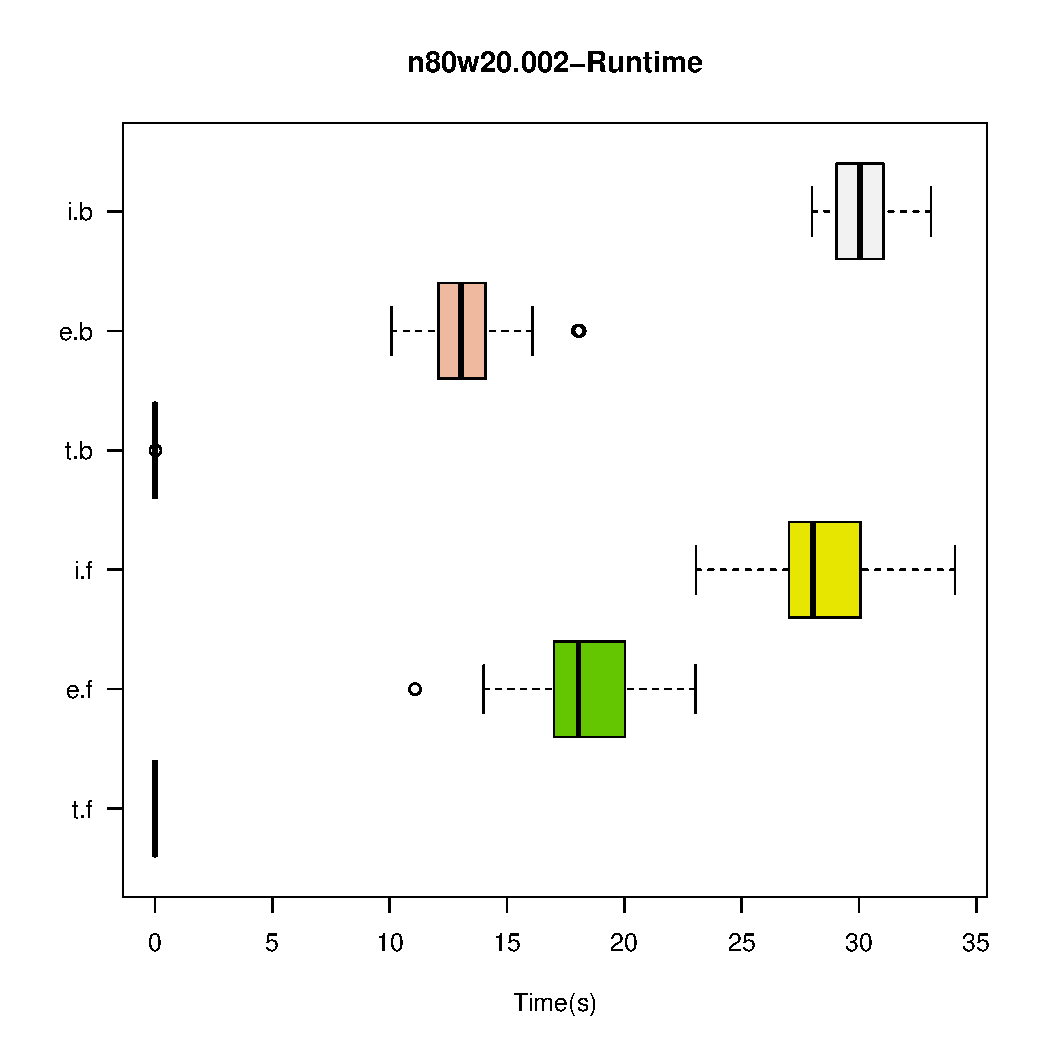
\includegraphics[width=0.6\textwidth,keepaspectratio]{{VND/n80w20.002/n80w20.002-CpuTime}.pdf}
\captionof{figure}{n80w20.002 - Runtime boxplots for the different variable neighborhood descent algorithms}
\end{center}

\begin{center}
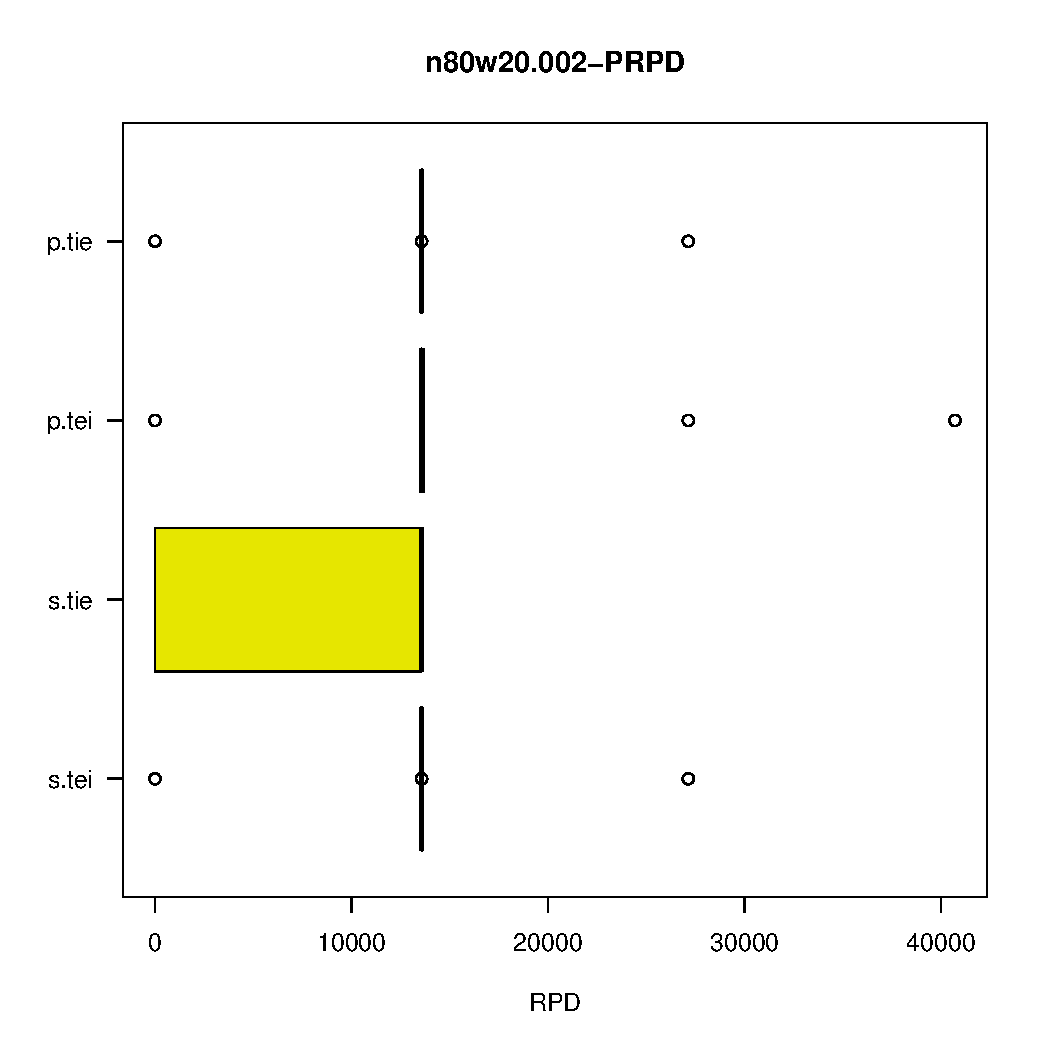
\includegraphics[width=0.6\textwidth,keepaspectratio]{{VND/n80w20.002/n80w20.002-PRPD}.pdf}
\captionof{figure}{n80w20.002 - PRPD boxplots for the different variable neighborhood descent algorithms}
\end{center}

\begin{center}
\begin{tabular}{|l|l|}
\hline
\textbf{Test} & \textbf{P-Value} \\
\hline
Tei vs Tie - Standard&3.9556885406462e-18\\
\hline
Tei vs Tie - Piped&3.95591160889952e-18\\
\hline
Standard vs Piped - Tei&3.95591160889952e-18\\
\hline
Standard vs Piped - Tie&3.95591160889952e-18\\
\hline
\end{tabular}
\captionof{table}{n80w20.002 - Results of Wilcoxon paired signed rank test}
\label{tab:w.12}
\end{center}

\subsubsection{n80w20.003}
\begin{center}
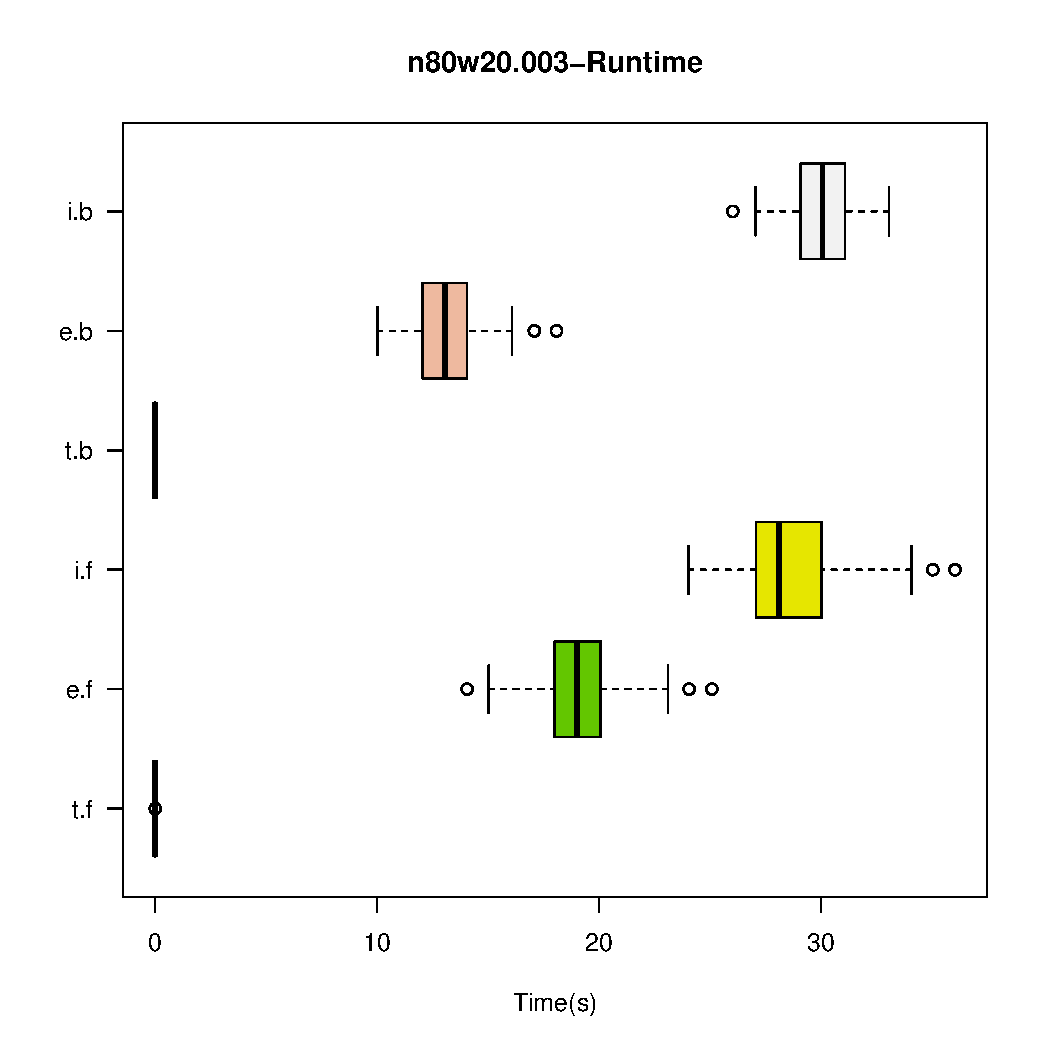
\includegraphics[width=0.6\textwidth,keepaspectratio]{{VND/n80w20.003/n80w20.003-CpuTime}.pdf}
\captionof{figure}{n80w20.003 - Runtime boxplots for the different variable neighborhood descent algorithms}
\end{center}

\begin{center}
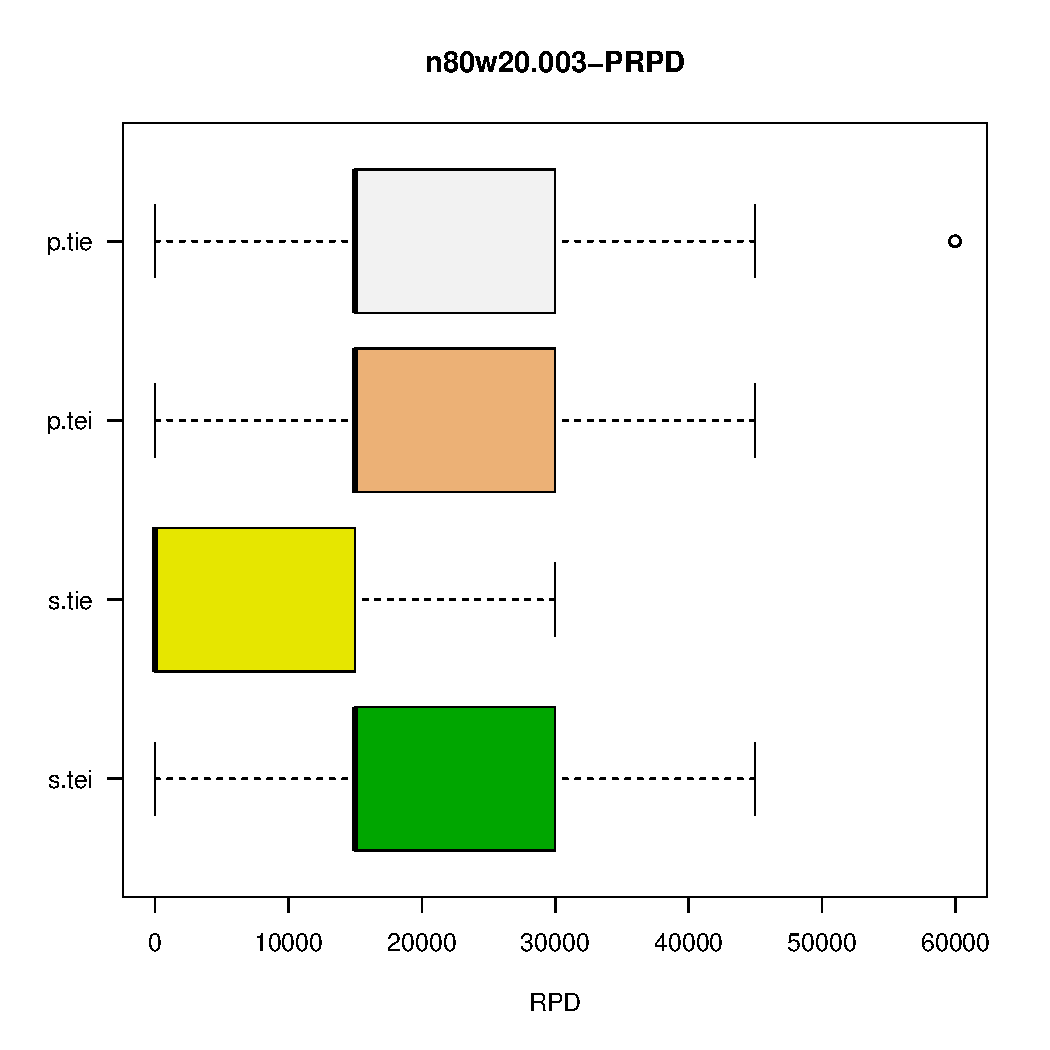
\includegraphics[width=0.6\textwidth,keepaspectratio]{{VND/n80w20.003/n80w20.003-PRPD}.pdf}
\captionof{figure}{n80w20.003 - PRPD boxplots for the different variable neighborhood descent algorithms}
\end{center}

\begin{center}
\begin{tabular}{|l|l|}
\hline
\textbf{Test} & \textbf{P-Value} \\
\hline
Tei vs Tie - Standard&3.9552424399092e-18\\
\hline
Tei vs Tie - Piped&3.95591160889952e-18\\
\hline
Standard vs Piped - Tei&3.95591160889952e-18\\
\hline
Standard vs Piped - Tie&3.95591160889952e-18\\
\hline
\end{tabular}
\captionof{table}{n80w20.003 - Results of Wilcoxon paired signed rank test}
\label{tab:w.13}
\end{center}

\subsubsection{n80w20.004}
\begin{center}
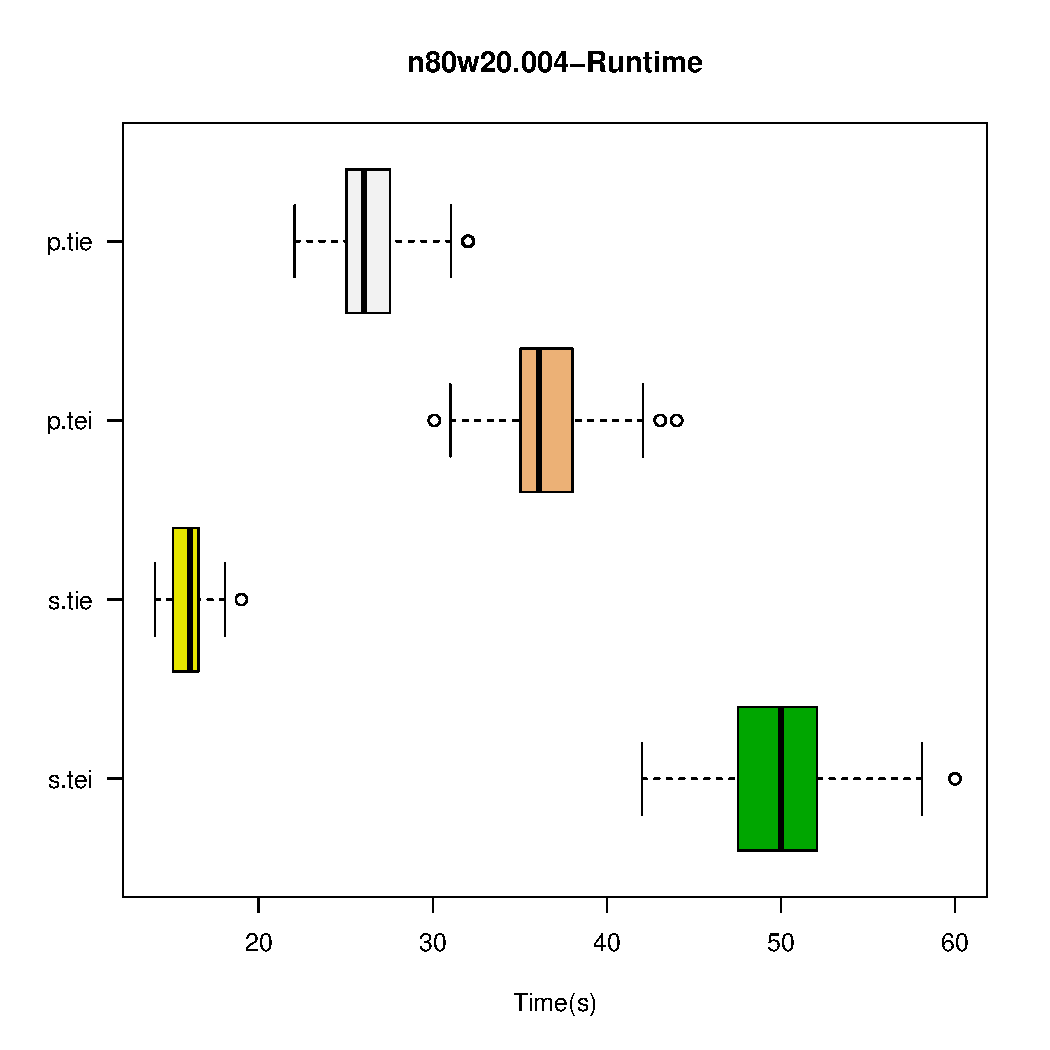
\includegraphics[width=0.6\textwidth,keepaspectratio]{{VND/n80w20.004/n80w20.004-CpuTime}.pdf}
\captionof{figure}{n80w20.004 - Runtime boxplots for the different variable neighborhood descent algorithms}
\end{center}

\begin{center}
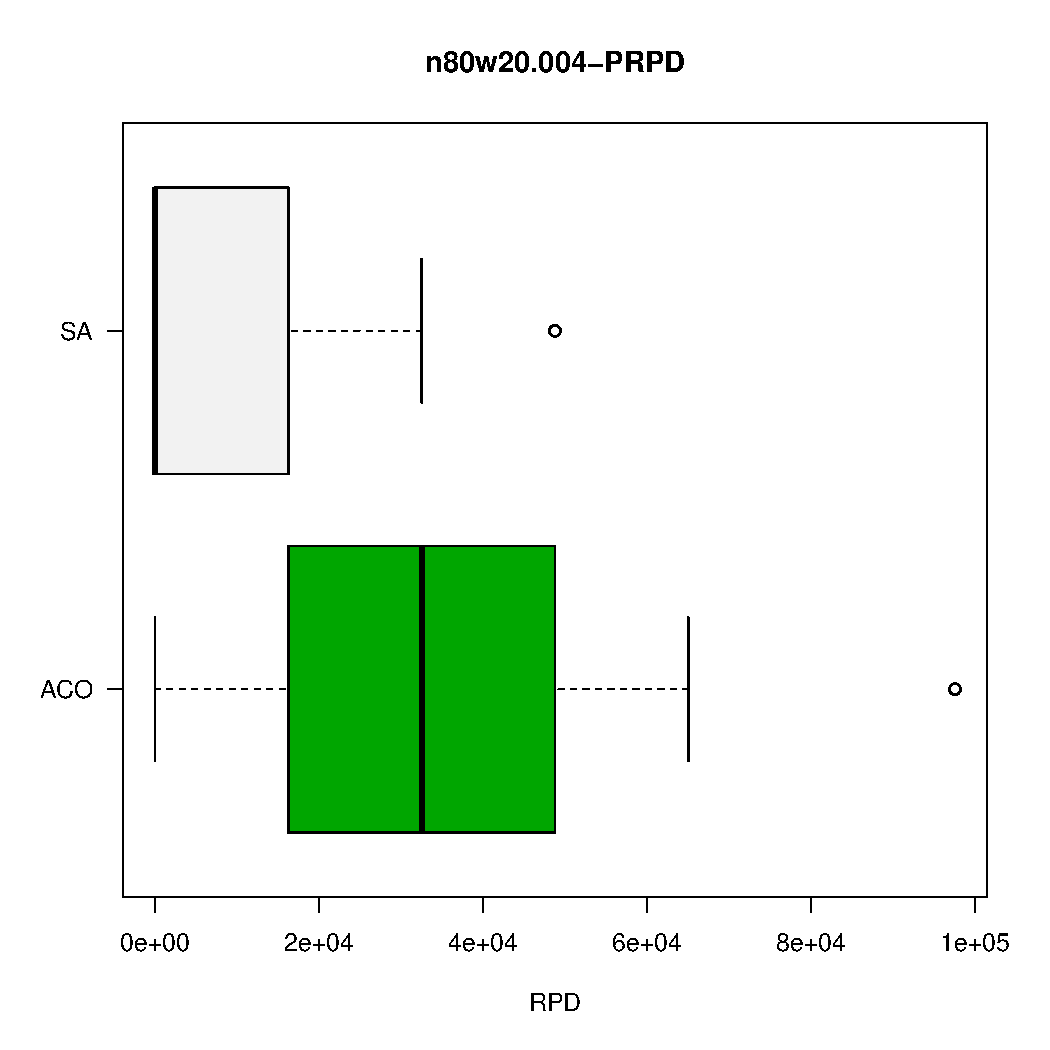
\includegraphics[width=0.6\textwidth,keepaspectratio]{{VND/n80w20.004/n80w20.004-PRPD}.pdf}
\captionof{figure}{n80w20.004 - PRPD boxplots for the different variable neighborhood descent algorithms}
\end{center}

\begin{center}
\begin{tabular}{|l|l|}
\hline
\textbf{Test} & \textbf{P-Value} \\
\hline
Tei vs Tie - Standard&3.95591160889952e-18\\
\hline
Tei vs Tie - Piped&3.95591160889952e-18\\
\hline
Standard vs Piped - Tei&3.95591160889952e-18\\
\hline
Standard vs Piped - Tie&3.95591160889952e-18\\
\hline
\end{tabular}
\captionof{table}{n80w20.004 - Results of Wilcoxon paired signed rank test}
\label{tab:w.14}
\end{center}

\subsubsection{n80w20.005}
\begin{center}
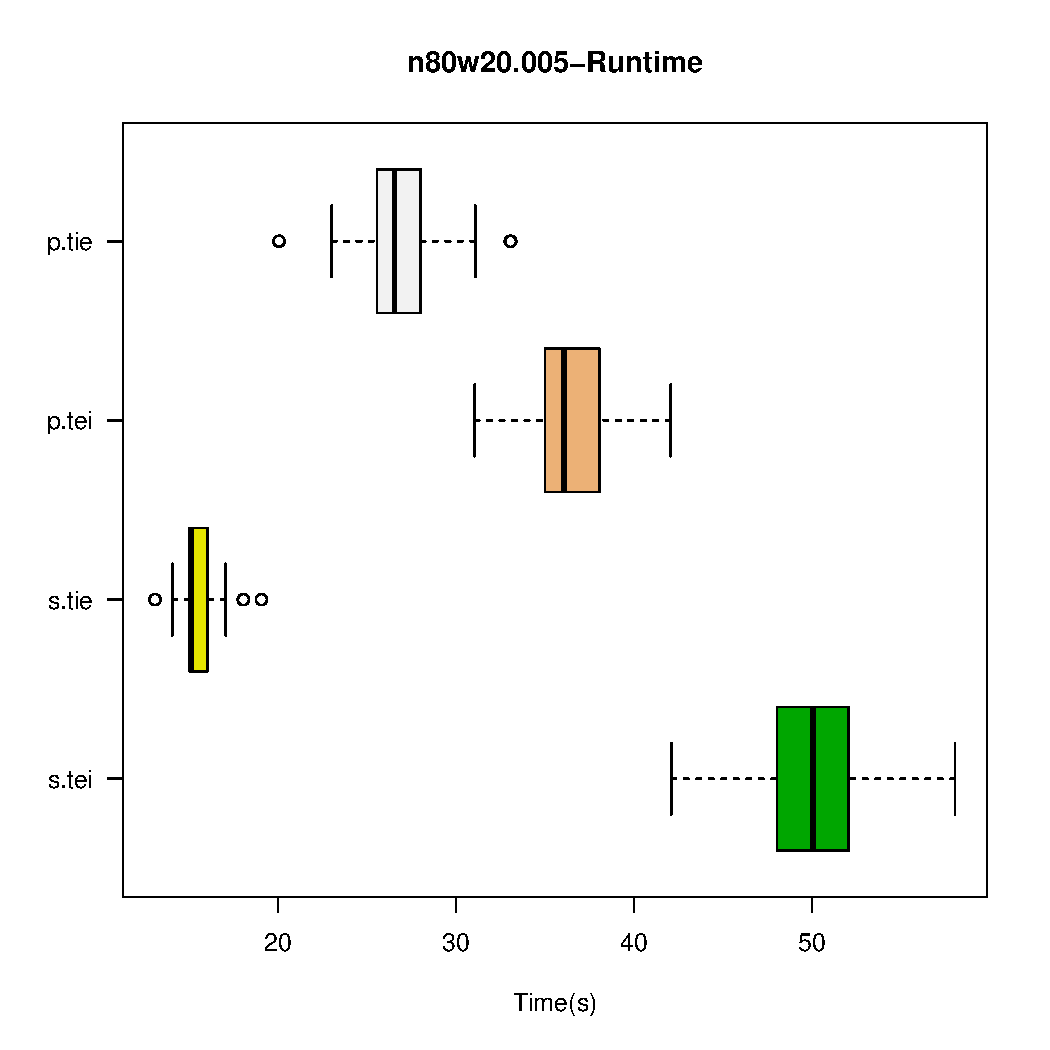
\includegraphics[width=0.6\textwidth,keepaspectratio]{{VND/n80w20.005/n80w20.005-CpuTime}.pdf}
\captionof{figure}{n80w20.005 - Runtime boxplots for the different variable neighborhood descent algorithms}
\end{center}

\begin{center}
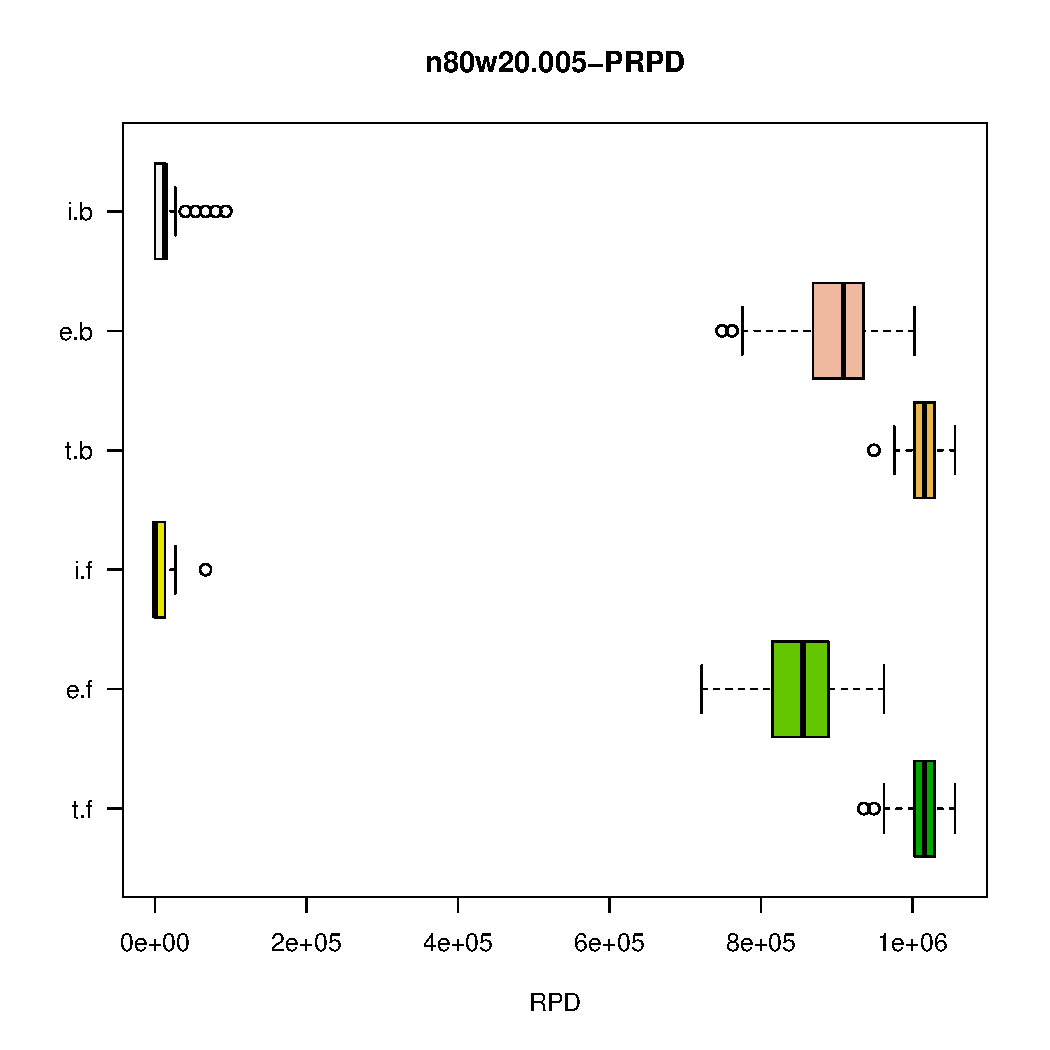
\includegraphics[width=0.6\textwidth,keepaspectratio]{{VND/n80w20.005/n80w20.005-PRPD}.pdf}
\captionof{figure}{n80w20.001 - PRPD boxplots for the different variable neighborhood descent algorithms}
\end{center}

\begin{center}
\begin{tabular}{|l|l|}
\hline
\textbf{Test} & \textbf{P-Value} \\
\hline
Tei vs Tie - Standard&3.95591160889952e-18\\
\hline
Tei vs Tie - Piped&3.95591160889952e-18\\
\hline
Standard vs Piped - Tei&3.95591160889952e-18\\
\hline
Standard vs Piped - Tie&3.95591160889952e-18\\
\hline
\end{tabular}
\captionof{table}{n80w20.005 - Results of Wilcoxon paired signed rank test}
\label{tab:w.15}
\end{center}

\subsubsection{n80w200.001}
\begin{center}
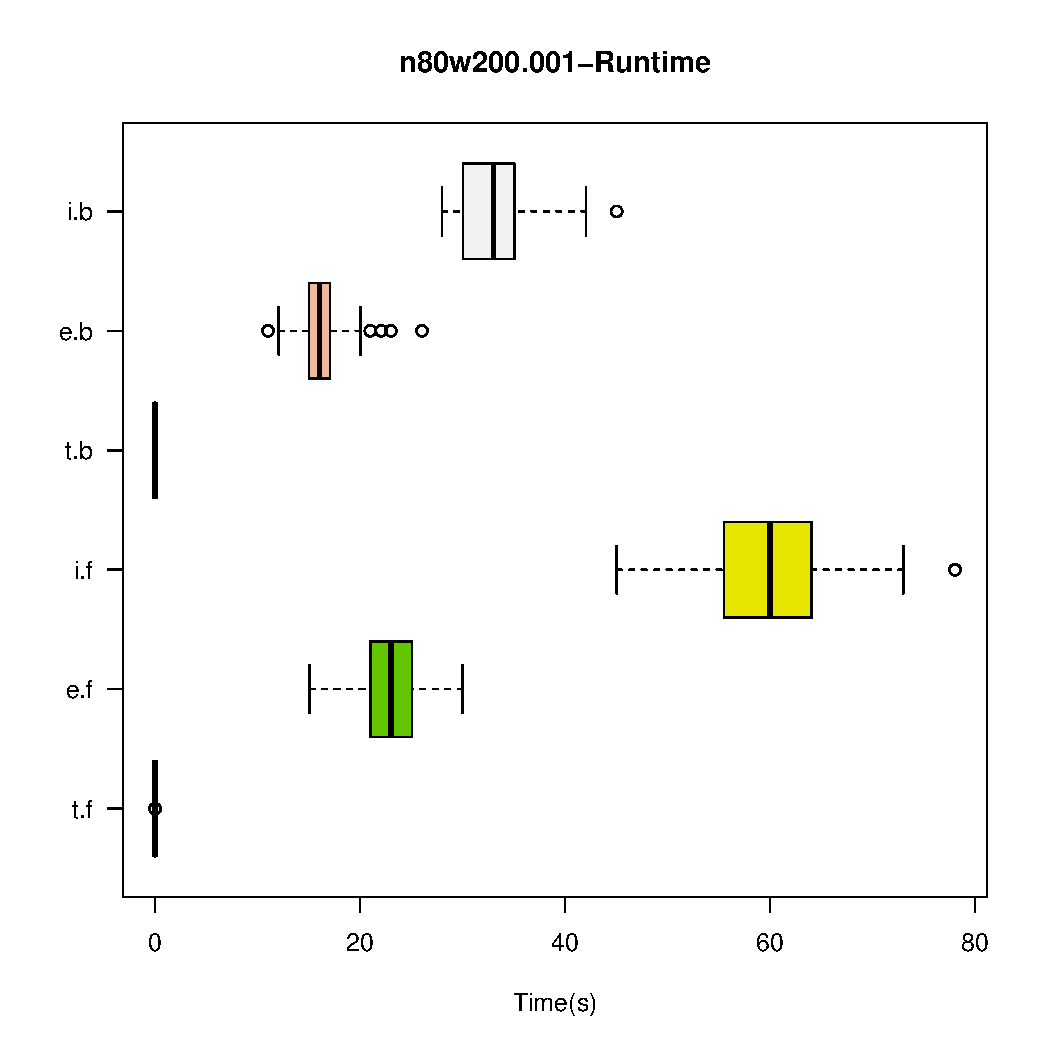
\includegraphics[width=0.6\textwidth,keepaspectratio]{{VND/n80w200.001/n80w200.001-CpuTime}.pdf}
\captionof{figure}{n80w200.001 - Runtime boxplots for the different variable neighborhood descent algorithms}
\end{center}

\begin{center}
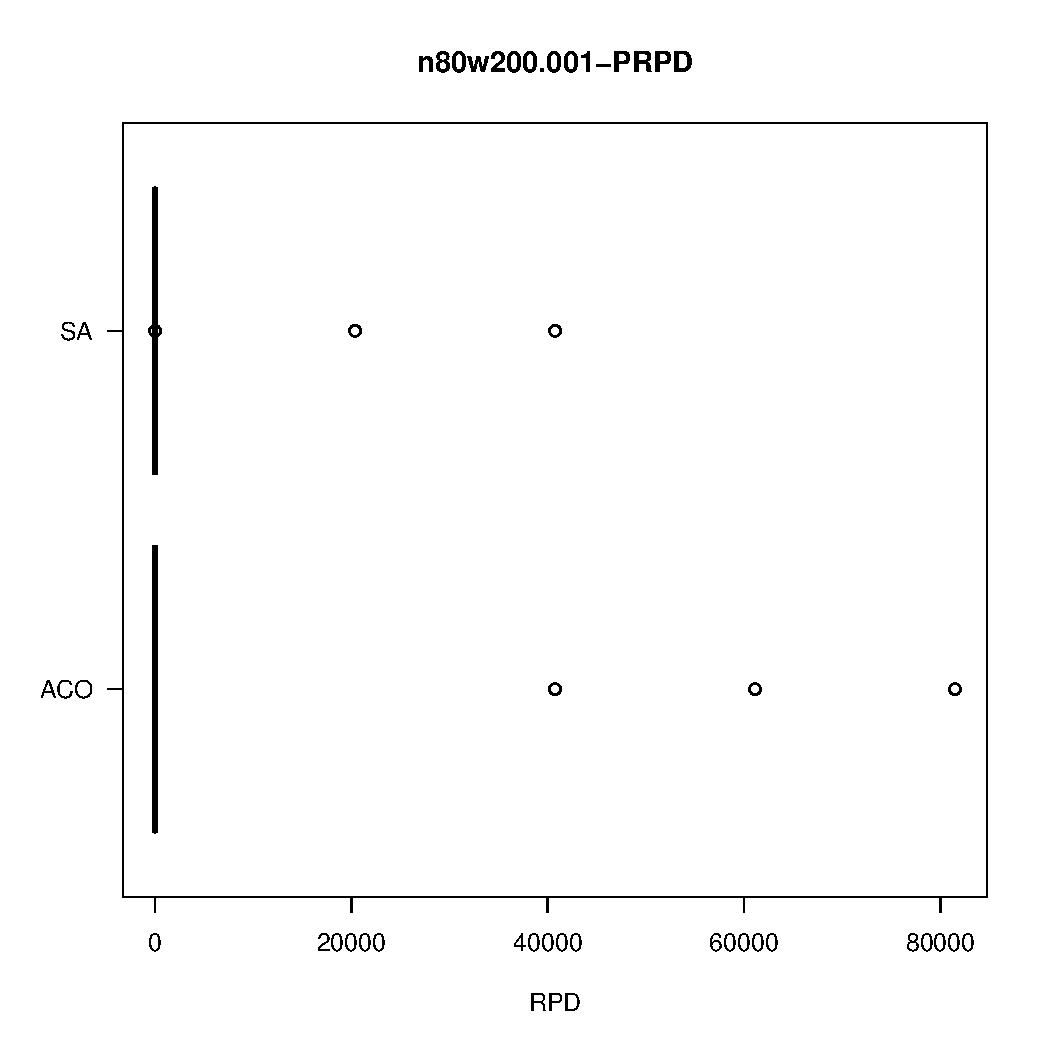
\includegraphics[width=0.6\textwidth,keepaspectratio]{{VND/n80w200.001/n80w200.001-PRPD}.pdf}
\captionof{figure}{n80w200.001 - PRPD boxplots for the different variable neighborhood descent algorithms}
\end{center}

\begin{center}
\begin{tabular}{|l|l|}
\hline
\textbf{Test} & \textbf{P-Value} \\
\hline
Tei vs Tie - Standard&4.07730530936212e-18\\
\hline
Tei vs Tie - Piped&2.92094064174088e-17\\
\hline
Standard vs Piped - Tei&2.72456795287507e-16\\
\hline
Standard vs Piped - Tie&3.95591160889952e-18\\
\hline
\end{tabular}
\captionof{table}{n80w200.001 - Results of Wilcoxon paired signed rank test}
\label{tab:w.16}
\end{center}

\subsubsection{n80w200.002}
\begin{center}
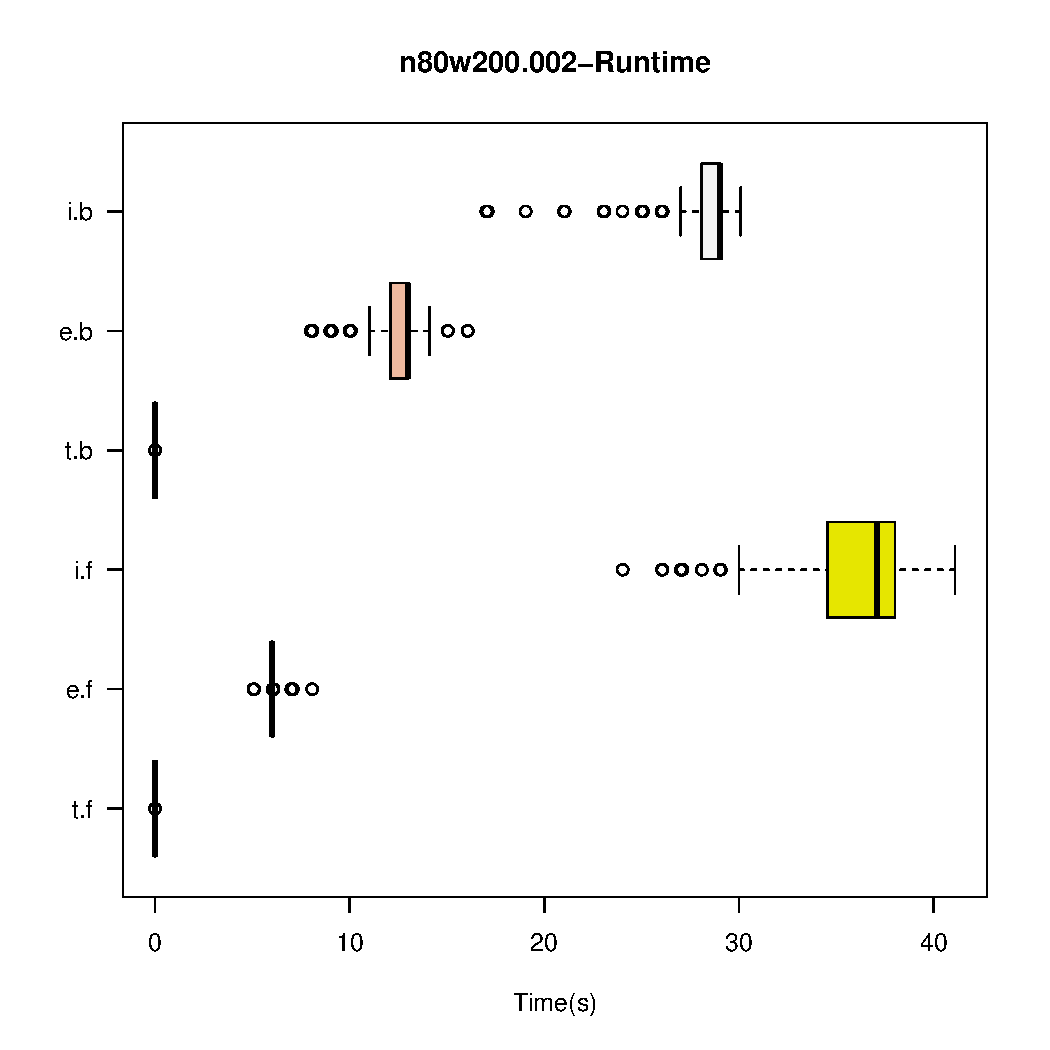
\includegraphics[width=0.6\textwidth,keepaspectratio]{{VND/n80w200.002/n80w200.002-CpuTime}.pdf}
\captionof{figure}{n80w200.002 - Runtime boxplots for the different variable neighborhood descent algorithms}
\end{center}

\begin{center}
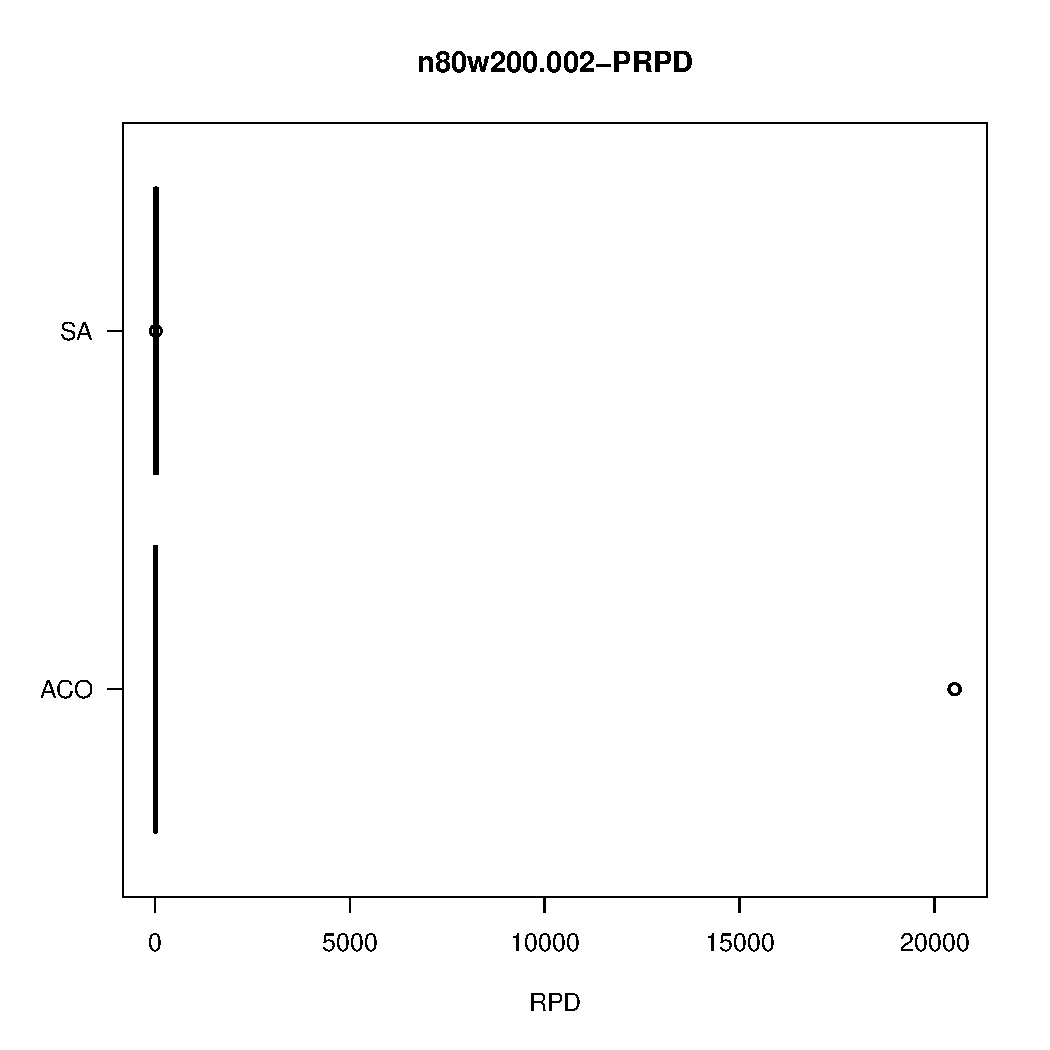
\includegraphics[width=0.6\textwidth,keepaspectratio]{{VND/n80w200.002/n80w200.002-PRPD}.pdf}
\captionof{figure}{n80w200.002 - PRPD boxplots for the different variable neighborhood descent algorithms}
\end{center}

\begin{center}
\begin{tabular}{|l|l|}
\hline
\textbf{Test} & \textbf{P-Value} \\
\hline
Tei vs Tie - Standard&3.95591160889952e-18\\
\hline
Tei vs Tie - Piped&1.52379449675399e-17\\
\hline
Standard vs Piped - Tei&1.74838327736385e-15\\
\hline
Standard vs Piped - Tie&3.95591160889952e-18\\
\hline
\end{tabular}
\captionof{table}{n80w200.002 - Results of Wilcoxon paired signed rank test}
\label{tab:w.17}
\end{center}

\subsubsection{n80w200.003}
\begin{center}
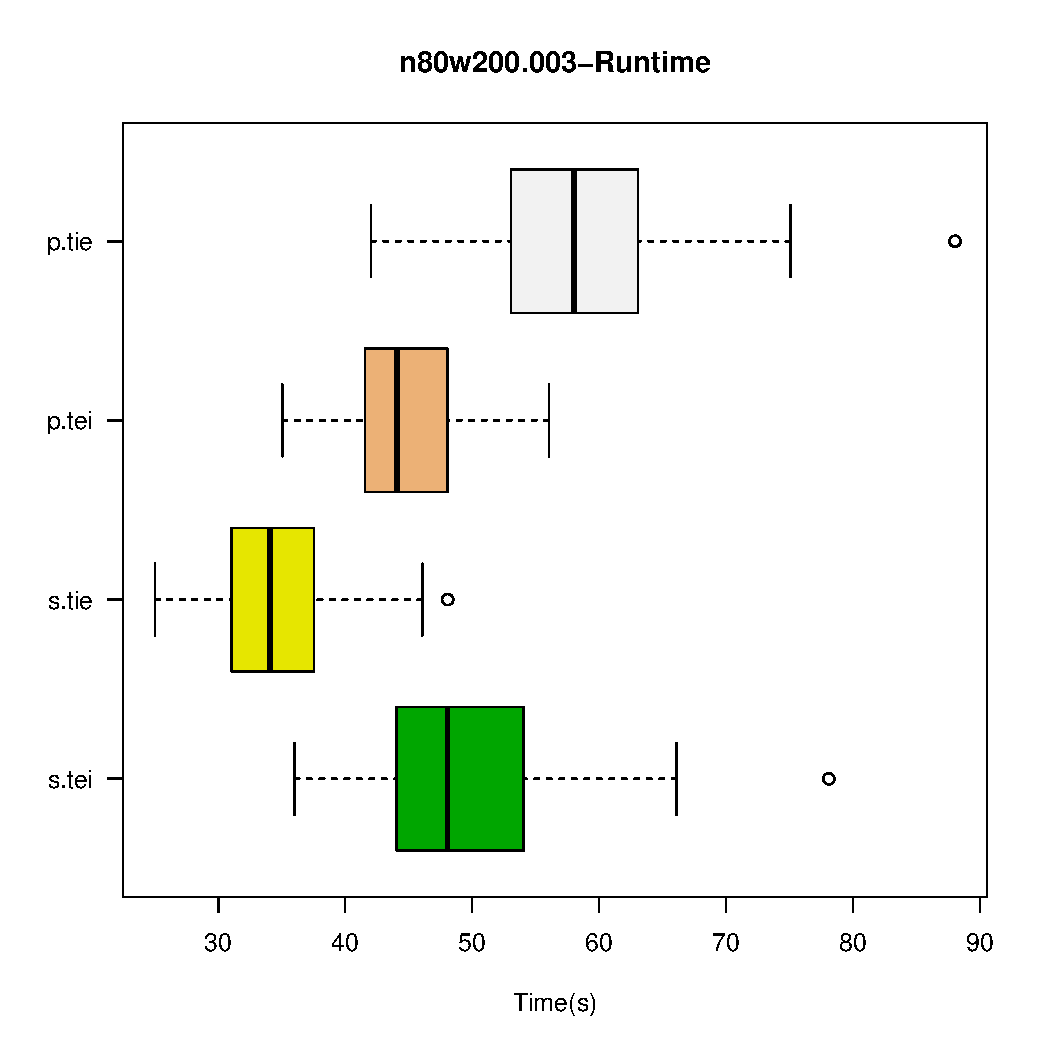
\includegraphics[width=0.6\textwidth,keepaspectratio]{{VND/n80w200.003/n80w200.003-CpuTime}.pdf}
\captionof{figure}{n80w200.003 - Runtime boxplots for the different variable neighborhood descent algorithms}
\end{center}

\begin{center}
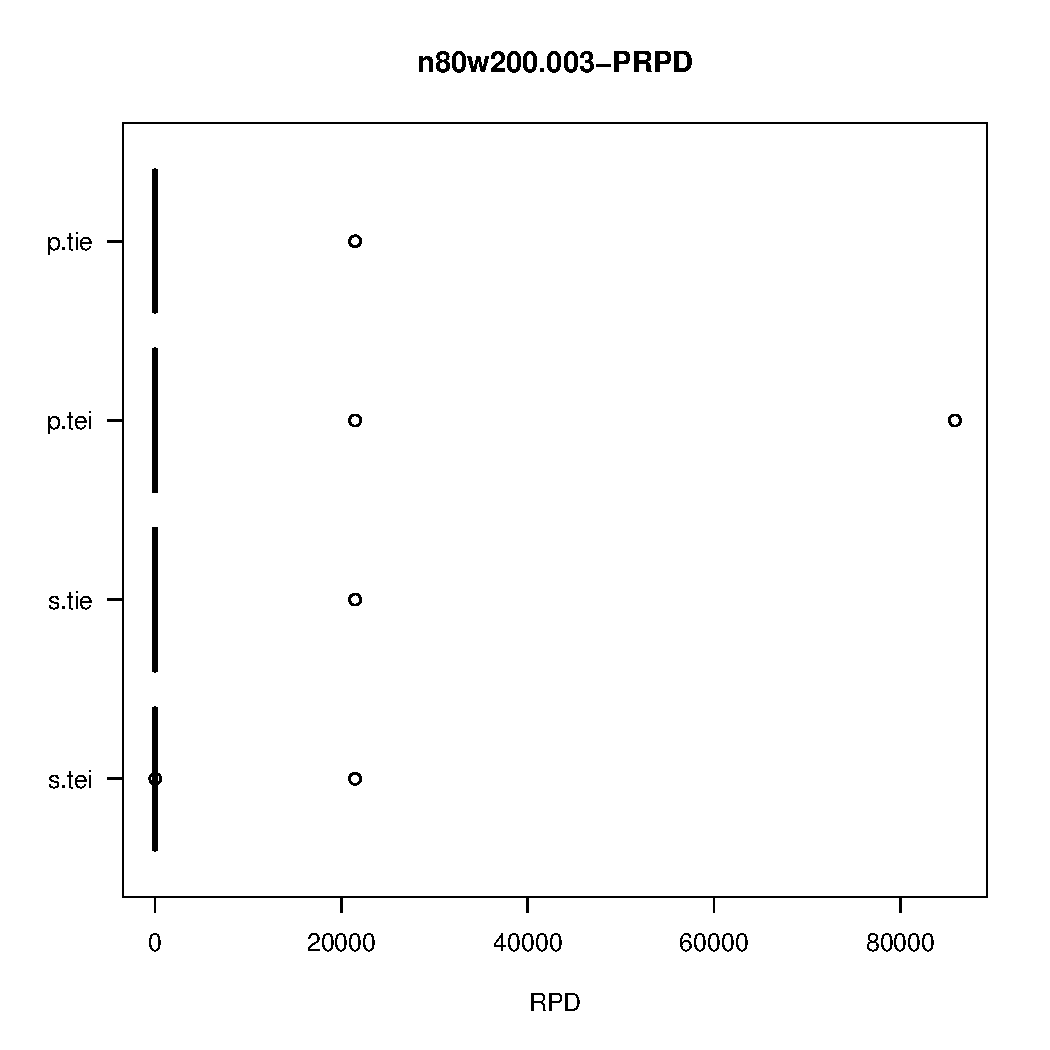
\includegraphics[width=0.6\textwidth,keepaspectratio]{{VND/n80w200.003/n80w200.003-PRPD}.pdf}
\captionof{figure}{n80w200.003 - PRPD boxplots for the different variable neighborhood descent algorithms}
\end{center}

\begin{center}
\begin{tabular}{|l|l|}
\hline
\textbf{Test} & \textbf{P-Value} \\
\hline
Tei vs Tie - Standard&2.04955667109233e-17\\
\hline
Tei vs Tie - Piped&2.59611565456869e-17\\
\hline
Standard vs Piped - Tei&1.50422804122146e-07\\
\hline
Standard vs Piped - Tie&3.95591160889952e-18\\
\hline
\end{tabular}
\captionof{table}{n80w200.003 - Results of Wilcoxon paired signed rank test}
\label{tab:w.18}
\end{center}

\subsubsection{n80w200.004}
\begin{center}
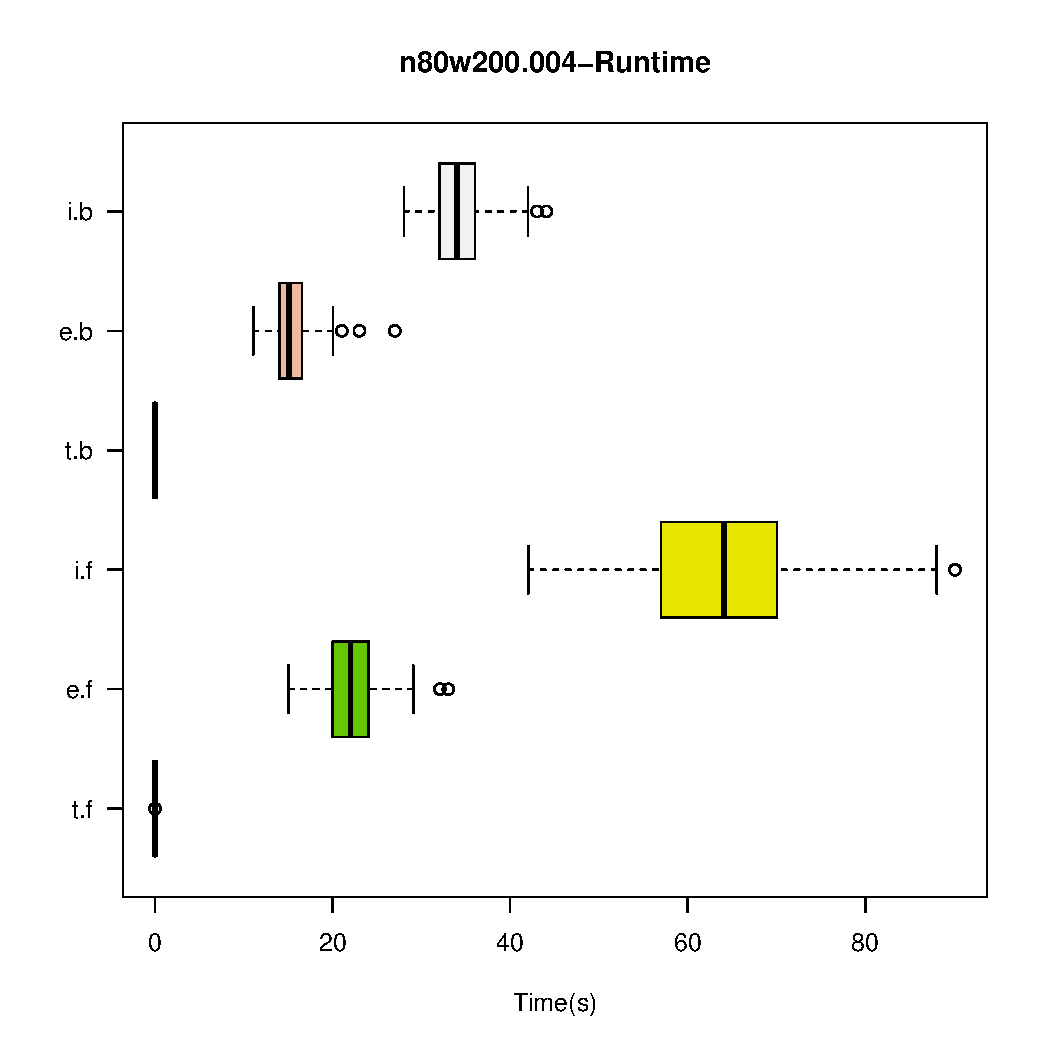
\includegraphics[width=0.6\textwidth,keepaspectratio]{{VND/n80w200.004/n80w200.004-CpuTime}.pdf}
\captionof{figure}{n80w200.004 - Runtime boxplots for the different variable neighborhood descent algorithms}
\end{center}

\begin{center}
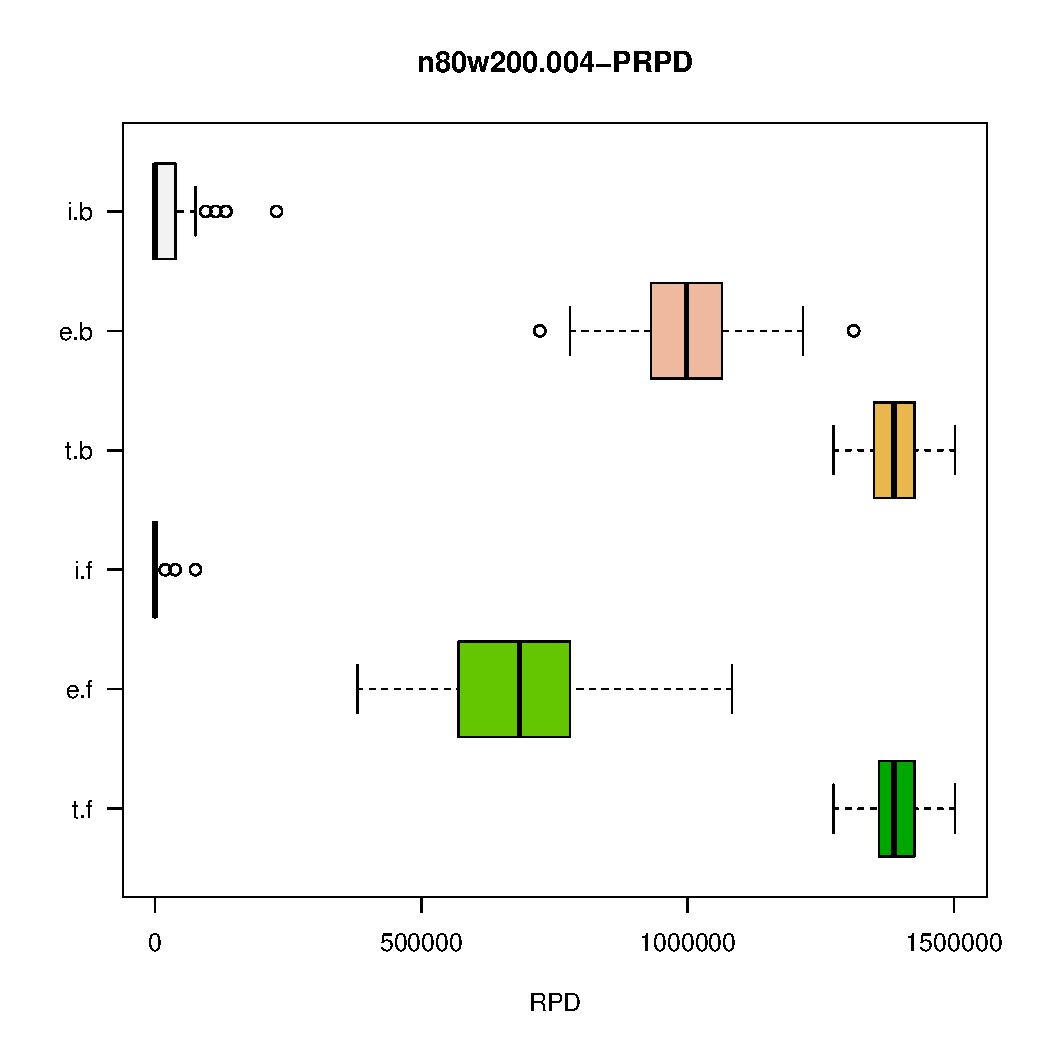
\includegraphics[width=0.6\textwidth,keepaspectratio]{{VND/n80w200.004/n80w200.004-PRPD}.pdf}
\captionof{figure}{n80w200.004 - PRPD boxplots for the different variable neighborhood descent algorithms}
\end{center}

\begin{center}
\begin{tabular}{|l|l|}
\hline
\textbf{Test} & \textbf{P-Value} \\
\hline
Tei vs Tie - Standard&4.07730530936212e-18\\
\hline
Tei vs Tie - Piped&4.29577057320019e-16\\
\hline
Standard vs Piped - Tei&5.3075517052254e-11\\
\hline
Standard vs Piped - Tie&3.95591160889952e-18\\
\hline
\end{tabular}
\captionof{table}{n80w200.004 - Results of Wilcoxon paired signed rank test}
\label{tab:w.19}
\end{center}

\subsubsection{n80w200.005}
\begin{center}
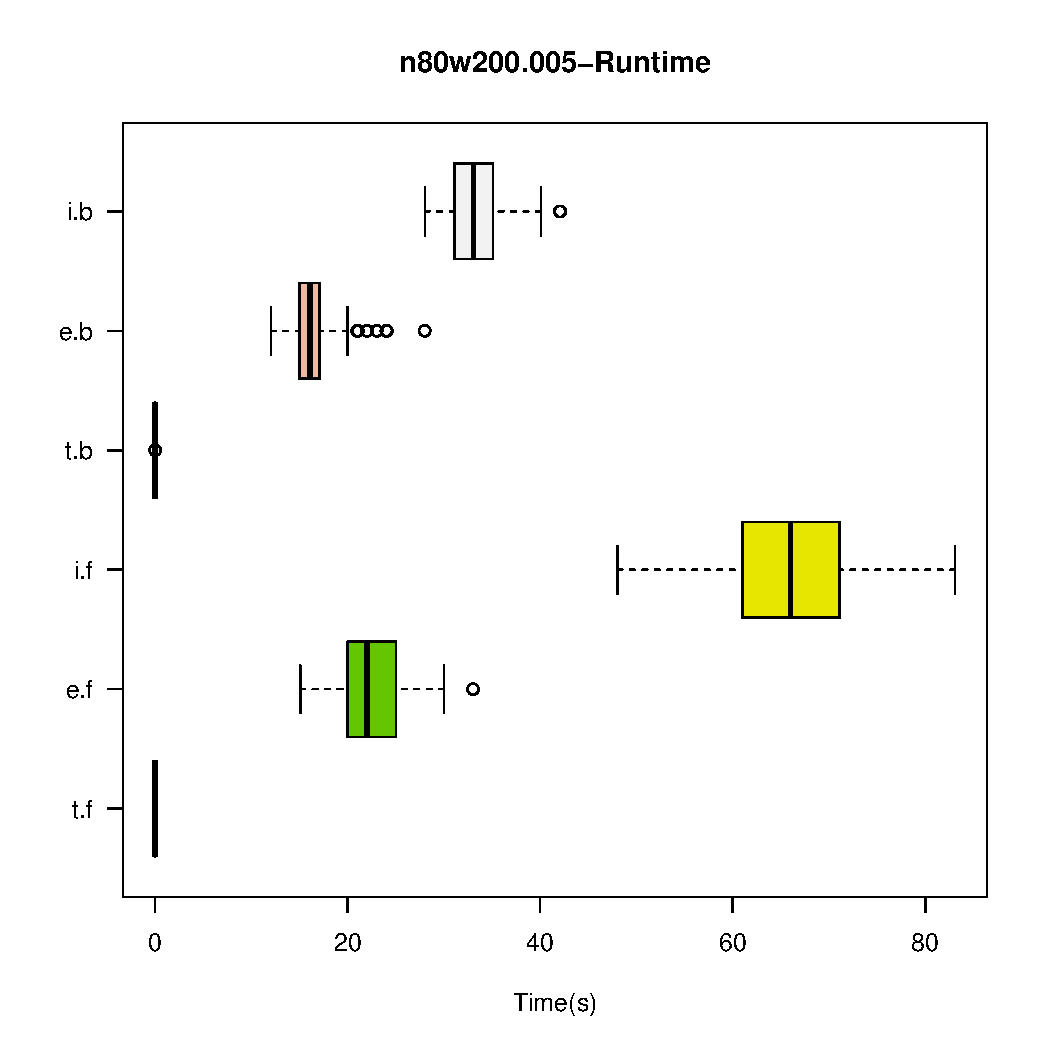
\includegraphics[width=0.6\textwidth,keepaspectratio]{{VND/n80w200.005/n80w200.005-CpuTime}.pdf}
\captionof{figure}{n80w200.005 - Runtime boxplots for the different variable neighborhood descent algorithms}
\end{center}

\begin{center}
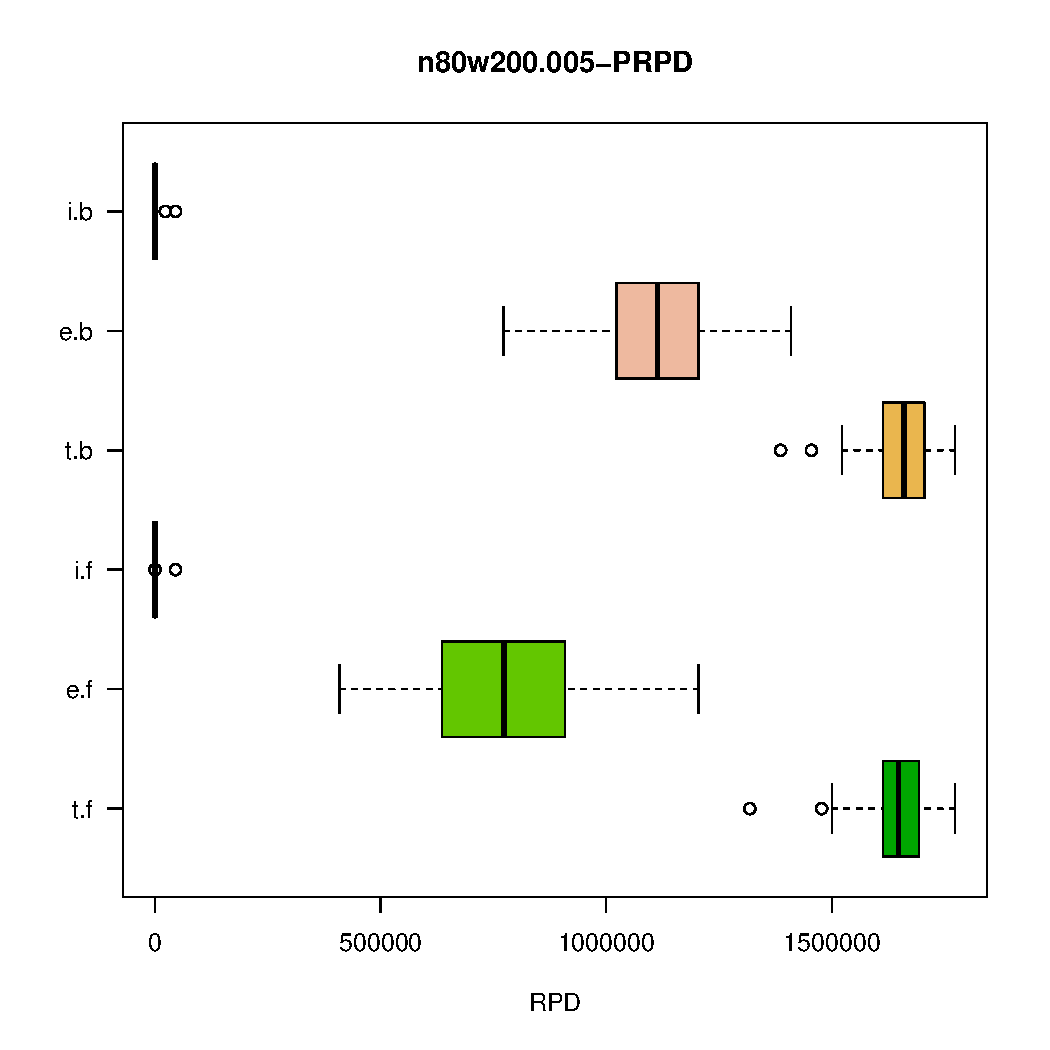
\includegraphics[width=0.6\textwidth,keepaspectratio]{{VND/n80w200.005/n80w200.005-PRPD}.pdf}
\captionof{figure}{n80w200.001 - PRPD boxplots for the different variable neighborhood descent algorithms}
\end{center}

\begin{center}
\begin{tabular}{|l|l|}
\hline
\textbf{Test} & \textbf{P-Value} \\
\hline
Tei vs Tie - Standard&1.39380002081336e-17\\
\hline
Tei vs Tie - Piped&4.07730530936212e-18\\
\hline
Standard vs Piped - Tei&3.72316935219101e-06\\
\hline
Standard vs Piped - Tie&3.95591160889952e-18\\
\hline
\end{tabular}
\captionof{table}{n80w200.001 - Results of Wilcoxon paired signed rank test}
\label{tab:w.20}
\end{center}

\subsection{Statistics}
\subsubsection{Standard-Transpose-Exchange-Insert}
\begin{center}
\begin{tabular}{|l|c|l|l|}
\hline
\textbf{Instance}& \textbf{\% Infeasible} & $\mathbf{\bar{PRDP}}$ &$\mathbf{\bar{Runtime}}$\\
\hline
n80w20.001&0.71&14772.04644164&50.611339\\
\hline
n80w20.002&0.88&12888.542&50.727053\\
\hline
n80w20.003&0.92&19936.872&50.820348\\
\hline
n80w20.004&0.62&17234.94260984&50.049484\\
\hline
n80w20.005&0.94&12564.0560428&50.269182\\
\hline
n80w200.001&0.28&11212.97389136&49.151249\\
\hline
n80w200.002&0.03&629.5853274&51.433949\\
\hline
n80w200.003&0.07&1511.56628539&49.082085\\
\hline
n80w200.004&0.16&4193.4817209&49.662512\\
\hline
n80w200.005&0.01&466.6729061&46.701953\\
\hline
\end{tabular}
\captionof{table}{Statistics summary for variable neighborhood descent algorithm with Transpose-Exchange-Insert neighborhood chain and Standard VND type}
\label{tab:s.tei}
\end{center}

\subsubsection{Standard-Transpose-Insert-Exchange}
\begin{center}
\begin{tabular}{|l|c|l|l|}
\hline
\textbf{Instance}& \textbf{\% Infeasible} & $\mathbf{\bar{PRDP}}$ &$\mathbf{\bar{Runtime}}$\\
\hline
n80w20.001&0.54&10874.77632472&15.268454\\
\hline
n80w20.002&0.62&8411.724&15.386641\\
\hline
n80w20.003&0.44&7645.295&15.638153\\
\hline
n80w20.004&0.39&7153.68881324&15.980347\\
\hline
n80w20.005&0.25&3475.2731712&15.55767\\
\hline
n80w200.001&0.16&4898.3227617&33.424555\\
\hline
n80w200.002&0&11.0430351&32.198479\\
\hline
n80w200.003&0.05&1082.1460308&34.345522\\
\hline
n80w200.004&0.28&7804.19186258&32.583152\\
\hline
n80w200.005&0&10.20227353&34.501294\\
\hline
\end{tabular}
\captionof{table}{Statistics summary for variable neighborhood descent algorithm with Transpose-Insert-Exchange neighborhood chain and Standard VND type}
\label{tab:s.tie}
\end{center}

\subsubsection{Piped-Transpose-Exchange-Insert}
\begin{center}
\begin{tabular}{|l|c|l|l|}
\hline
\textbf{Instance}& \textbf{\% Infeasible} & $\mathbf{\bar{PRDP}}$ &$\mathbf{\bar{Runtime}}$\\
\hline
n80w20.001&0.59&12336.84228578&35.694416\\
\hline
n80w20.002&0.94&15603.0142035&36.212393\\
\hline
n80w20.003&0.83&19338.924&34.821217\\
\hline
n80w20.004&0.55&13170.33921962&36.438959\\
\hline
n80w20.005&0.45&6683.336214&36.202891\\
\hline
n80w200.001&0.19&5104.3621015&40.772642\\
\hline
n80w200.002&0.01&218.8179842&44.241593\\
\hline
n80w200.003&0.06&2584.90674231&44.725066\\
\hline
n80w200.004&0.17&3430.64506042&43.760992\\
\hline
n80w200.005&0.02&693.0136326&42.646023\\
\hline
\end{tabular}
\captionof{table}{Statistics summary for variable neighborhood descent algorithm with Transpose-Exchange-Insert neighborhood chain and Piped VND type}
\label{tab:p.tei}
\end{center}

\subsubsection{Piped-Transpose-Insert-Exchange}
\begin{center}
\begin{tabular}{|l|c|l|l|}
\hline
\textbf{Instance}& \textbf{\% Infeasible} & $\mathbf{\bar{PRDP}}$ &$\mathbf{\bar{Runtime}}$\\
\hline
n80w20.001&0.68&16393.81210394&24.788225\\
\hline
n80w20.002&0.81&11667.654&25.902581\\
\hline
n80w20.003&0.84&20537.669&26.442309\\
\hline
n80w20.004&0.46&8779.79314651&26.424231\\
\hline
n80w20.005&0.24&3876.3661498&26.511156\\
\hline
n80w200.001&0.21&5917.0312803&52.302366\\
\hline
n80w200.002&0.01&626.0983757&56.238843\\
\hline
n80w200.003&0.04&867.92563269&58.498874\\
\hline
n80w200.004&0.28&6281.58944822&55.867038\\
\hline
n80w200.005&0.01&236.8657243&58.331595\\
\hline
\end{tabular}
\captionof{table}{Statistics summary for variable neighborhood descent algorithm with Transpose-Insert-Exchange neighborhood chain and Piped VND type}
\label{tab:p.tie}
\end{center}

\subsection{Results discussion}
By looking at tables \ref{tab:s.tei}, \ref{tab:s.tie}, \ref{tab:p.tei}, \ref{tab:p.tie} one can see that:
\begin{itemize}

\item For some instances (e.g. $n80w20.002$,$n80w20.003$) the algorithm are not able to converge to a feasible solution, as shown in the corresponding boxplots, since the PRPD distribution is centered around 12000-15000, thus indicating the presence of at least 1 constraint violations in most of the cases.

\item For some other instances (e.g. $n80w20.004$,$n80w20.005$) the algorithms are able to converge to feasible solutions and to the best-known one, but having a right-skewed distribution towards higher values of PRPD.

\item For the remaining instances, except for some outlier values, the algorithms are able to converge to the best-known solution in most of the runs , even though the average PRPD is not closer to 0. This is due to the fact that the mean of a distribution is sensible to outliers and the penalisation for a constraint violations is extremely high when compared to the mean value.
      
\item The algorithm ordering in terms of runtimes is $s.tie < p.tie < p.tei < s.tei$ for the  $n80w20.X$ instances while $s.tie < p.tei < s.tei < p.tie$ for $n80w200.X$ ones. The choice to explore the Insert Neighborhood before the Exchange one allows to reduce the computation time for the $n80w20.X$ instances, with a similar solution quality.

\item The algorithms are more effective on the $n80w200.X$ instances then the $n80w20.X$ once, since they have a lower percentage of infeasible runs and a lower PRPD.

\item The standard variable neighborhood descent with Transpose-Insert-Exchange neighborhood chain (s.tie) outperforms all the other algorithms in terms of solution quality and runtime.

\item Tables \ref{tab:w.11}, \ref{tab:w.12}, \ref{tab:w.13}, \ref{tab:w.14}, \ref{tab:w.15}, \ref{tab:w.16}, \ref{tab:w.17}, \ref{tab:w.18}, \ref{tab:w.19}, \ref{tab:w.20} contain, in any case, p-values considerably smaller than the significance level ($\alpha=0.05$). 

This implies that the null hypothesis corresponding to the equality of the median values of the differences of the two distributions can be rejected, hence assessing the existence of a statistically significant difference among the solution quality generated by analyzed algorithms.

\item By looking at the Cpu time, one can see that the instances \emph{n80w20.X} have generally lower runtimes than the \emph{n80w200.X} ones. They can then be considered, with respect to the variable neighborhood descent algorithms, simpler (quickier to solve) instances with respect to the latter.

\end{itemize}

\end{homeworkProblem}
